\section{FMU Examples}\label{fmu-examples}

\subsection{Architecture of the FMU for co-simulation Import}\label{architecture-of-the-fmu-for-co-simulation-import}

Figure~\ref{fig:architecture-of-the-fmu-for-co-simulation} shows the architecture of the connection between EnergyPlus and two FMUs. EnergyPlus imports the FMUs that connect to its external interface. These FMUs are generated by external simulation environments that implement the FMI Application Programming Interface (API) for co-simulation. See \url{http://www.modelisar.com/tools.html} for a list of programs that export FMUs. In the external interface, the input/output signals that are exchanged between the FMUs and EnergyPlus are mapped to EnergyPlus objects. The subject of this External Interface Application Guide is how to configure this mapping and how to use these objects.

\begin{figure}[hbtp] % fig 9
\centering
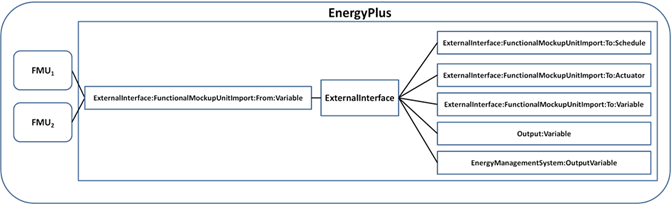
\includegraphics[width=0.9\textwidth, height=0.9\textheight, keepaspectratio=true]{media/image035.png}
\caption{Architecture of the FMU for co-simulation import. \protect \label{fig:architecture-of-the-fmu-for-co-simulation}}
\end{figure}

The external interface can map to three EnergyPlus input objects called

\begin{itemize}
\item
  ExternalInterface:FunctionalMockupUnitImport:To:Schedule
\item
  ExternalInterface:FunctionalMockupUnitImport:To:Actuator
\item
  ExternalInterface:FunctionalMockupUnitImport:To:Variable.
\end{itemize}

The ExternalInterface:FunctionalMockupUnitImport:To:Schedule can be used to overwrite schedules, and the other two objects can be used in place of Energy Management System (EMS) actuators and EMS variables. The objects have similar functionality as the objects Schedule:Compact, EnergyManagementSystem:Actuator and EnergyManagementSystem:GlobalVariable, except that their numerical value is obtained from the external interface at the beginning of each zone time step, and will remain constant during this zone time step.

The external interface also uses the ExternalInterface:FunctionalMockupUnitImport:From:Variable object which~ maps to EnergyPlus objects Output:Variable and EnergyManagementSystem:OutputVariable to send data from EnergyPlus to FMUs at each zone time step.

We will now present examples that use all of these objects. The following table shows which EnergyPlus features are used in the examples.

% table 3
\begin{longtable}[c]{p{1.5in}p{1.5in}p{1.5in}p{1.5in}}
\caption{Overview of the EnergyPlus objects used in Examples \label{table:overview-of-the-energyplus-objects-used-in-001}} \tabularnewline
\toprule 
~ & Example 1 & Example 2 & Example 3 \tabularnewline
\midrule
\endfirsthead

\caption[]{Overview of the EnergyPlus objects used in Examples} \tabularnewline
\toprule 
~ & Example 1 & Example 2 & Example 3 \tabularnewline
\midrule
\endhead

ExternalInterface:FunctionalMockupUnitImport:From:Variable & x & x & x \tabularnewline
ExternalInterface:FunctionalMockupUnitImport:To:Schedule & x & ~ & ~ \tabularnewline
ExternalInterface:FunctionalMockupUnitImport:To:Actuator & ~ & x & ~ \tabularnewline
ExternalInterface:FunctionalMockupUnitImport:To:Variable & ~ & ~ & x \tabularnewline
Output:Variable & x & x & x \tabularnewline
\bottomrule
\end{longtable}

Prior to discussing the examples, we will explain the pre-processing steps that are required to prepare EnergyPlus to be linked to FMUs for co-simulation.

\subsection{Workflow of the FMU for co-simulation import}\label{workflow-of-the-fmu-for-co-simulation-import}

To use the FMU for co-simulation import, there are two important steps: pre-processing and co-simulation.~ The pre-processing step generates a section of an EnergyPlus input file (*.idf) that can be used to configure the FMU for co-simulation import. The input file defines the input and output variables for both EnergyPlus and FMUs. The co-simulation step performs co-simulation.

Figure~\ref{fig:work-flow-for-pre-processing.} shows the work flow for pre-processing. First, a FMU Parser parses the FMU files (i.e.~xxx.fmu) and generates a temporary EnergyPlus input file (i.e.~xxxtmp.idf). The temporary EnergyPlus input file is not complete as it just contains information related to the FMU, such as names of the FMU and properties of each FMU variable including variable name, associated FMU name, input/output type, data type, units and definitions. The user will need to manually copy the FMU information from xxxtmp.idf into the EnergyPlus input file xxx.idf. The user then needs to modify the xxx.idf file to link the FMU variables with EnergyPlus variables.

\begin{figure}[hbtp] % fig 10
\centering
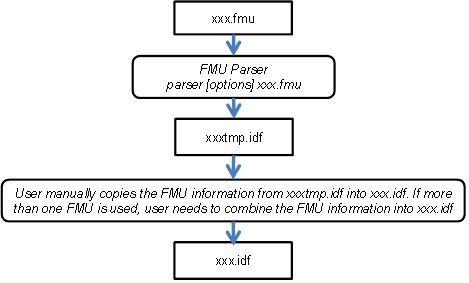
\includegraphics[width=0.9\textwidth, height=0.9\textheight, keepaspectratio=true]{media/image036.png}
\caption{Work flow for pre-processing. \protect \label{fig:work-flow-for-pre-processing.}}
\end{figure}

\subsection{FMU Parser}\label{fmu-parser}

The FMU parser is a code written in C. It includes Expat (Expat XML Parser, 2011) which is a XML parser library written in C. The low level implementation of the function (\emph{parser}) that is used to process a FMU is \emph{parser {[}options{]} xxx.fmu}, where \emph{options} are as follows:

\begin{itemize}
\item
  \emph{--printidf}, prints a temporary xxxtmp.idf with FMU information to be printed,
\item
  \emph{--unpack}, unpacks a FMU to be unpacked, and
\item
  \emph{--delete}, deletes temporary files related to FMUs.
\end{itemize}

A FMU is a zip file which may contain executable programs for specific platforms, description files and source code. In the pre-processing step, the FMU Parser will be called with the command option \emph{--printidf.} This will cause the parser to parse the XML file with the model description of the FMU and write the FMU information in a format of the EnergyPlus input file (*.idf). The parser will check if all the required fields from FMU (see next section for details) in the *.idf file are correctly specified. If the check succeeds, the parser will successfully close. If the check fails, the parser will close with an error message. After the EnergyPlus executable (such as EnergyPlus.exe) terminates, the EnergyPlus batch file will delete all the temporary files that may have been generated.~~ The FMU Parser is distributed with EnergyPlus and can be found in the PreProcess folder (FMUParser) of the EnergyPlus installation.

\textbf{~}

\begin{figure}[hbtp] % fig 11
\centering
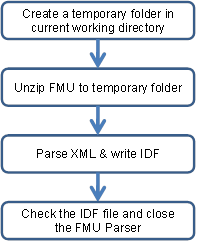
\includegraphics[width=0.9\textwidth, height=0.9\textheight, keepaspectratio=true]{media/image037.png}
\caption{Workflow of FMU parser for pre-processing. \protect \label{fig:workflow-of-fmu-parser-for-pre-processing.}}
\end{figure}

\subsection{Example 1: Interface using ExternalInterface:FunctionalMockupUnitImport:To:Schedule}\label{example-1-interface-using-externalinterfacefunctionalmockupunitimporttoschedule}

In this example, an HVAC system implemented in a FMU (MoistAir.fmu) is linked to a room model in EnergyPlus. The HVAC system computes sensible and latent heat gain required for maintaining a set point temperature. The FMU needs as input the outdoor dry-bulb (TDryBul) temperature, outdoor air relative humidity (outRelHum), the room dry-bulb temperature (TRooMea) and the room air relative humidity (rooRelHum). The outputs of the FMU are the latent (QLatent) and sensible (QSensible) heat transported across the thermodynamic boundary of air inlet and outlet of the thermal zone.

To link the FMU with EnergyPlus, we need to send from the FMU to EnergyPlus two schedule values for the latent and sensible heat gain and from EnergyPlus to the FMU four output variables for outdoor dry-bulb temperature, outdoor air relative humidity, room dry-bulb temperature and room air relative humidity at each zone time step. This can be accomplished by using two objects of type ExternalInterface:FunctionalMockupUnitImport:To:Schedule and four objects of type ExternalInterface:FunctionalMockupUnitImport:From:Variable.

To interface EnergyPlus, the following four items are needed:

\begin{itemize}
\item
  An object that instructs EnergyPlus to activate the external interface.
\item
  An object that specifies the FMU and its instances.
\item
  EnergyPlus objects that read data from EnergyPlus and send to FMU.
\item
  EnergyPlus objects that read data from FMU and send to EnergyPlus.
\end{itemize}

\subsubsection{Creating the EnergyPlus idf file}\label{creating-the-energyplus-idf-file-000}

To create the EnergyPlus idf file the user should:

\begin{itemize}
\item
  Use the \emph{parser} to generate a temporary idf.
\item
  Copy the FMU information from the temporary idf into the full idf file.
\item
  Modify the full idf file to link the FMU variables with EnergyPlus variables.
\end{itemize}

The code below shows how the objects will be in the idf.

To activate the external interface, we use:

\begin{lstlisting}

ExternalInterface,           !- Object to activate the external interface
   FunctionalMockupUnitImport; !- Name of external interface
\end{lstlisting}

To define the FMU that will be linked to EnergyPlus, we use:

\begin{lstlisting}

ExternalInterface:FunctionalMockupUnitImport,
      MoistAir.fmu,            !- FMU Filename
      15,                       !- FMU Timeout
      0;                        !- FMU LoggingOn
\end{lstlisting}

To enter output variables from which the external interface read and send to FMUs, we use:

\begin{lstlisting}

ExternalInterface:FunctionalMockupUnitImport:From:Variable,
      Environment,                      !- EnergyPlus Key Value
      Site Outdoor Air Drybulb Temperature,     !- EnergyPlus Variable Name
      MoistAir.fmu,                     !- FMU Filename
      Model1,                           !-FMU Model Name
      TDryBul;                          !- FMU Model Variable Name


  ExternalInterface:FunctionalMockupUnitImport:From:Variable,
      ZONE ONE,                         !- EnergyPlus Key Value
      Zone Mean Air Temperature,        !- EnergyPlus Variable Name
      MoistAir.fmu,                     !- FMU Filename
      Model1,                           !- FMU Model Name
      TRooMea;                          !- FMU Model Variable Name


  ExternalInterface:FunctionalMockupUnitImport:From:Variable,
      Environment,                      !- EnergyPlus Key Value
      Site Outdoor Air Relative Humidity,      !- EnergyPlus Variable Name
      MoistAir.fmu,                     !- FMU Filename
      Model1,                           !- FMU Model Name
      outRelHum;                        !- FMU Model Variable Name


  ExternalInterface:FunctionalMockupUnitImport:From:Variable,
      ZONE ONE,                         !- EnergyPlus Key Value
      Zone Air Relative Humidity,       !- EnergyPlus Variable Name
      MoistAir.fmu,                     !- FMU Filename
      Model1,                           !- FMU Model Name
      rooRelHum;                        !- FMU Model Variable Name
\end{lstlisting}

These output variables need to be specified in the idf file:

\begin{lstlisting}

Output:Variable,
      Environment,                 !- Key Value
      Site Outdoor Air Drybulb Temperature,            !- Variable Name
      TimeStep;                    !- Reporting Frequency


  Output:Variable,
      ZONE ONE,                    !- Key Value
      Zone Mean Air Temperature,   !- Variable Name
      TimeStep;                    !- Reporting Frequency


  Output:Variable,
      Environment,                 !- Key Value
      Site Outdoor Air Relative Humidity,   !- Variable Name
      TimeStep;                    !- Reporting Frequency


  Output:Variable,
      ZONE ONE,                    !- Key Value
      Zone Air Relative Humidity,  !- Variable Name
      TimeStep;                    !- Reporting Frequency
\end{lstlisting}

To enter schedules to which the external interface writes, we use:

\begin{lstlisting}

ExternalInterface:FunctionalMockupUnitImport:To:Schedule,
      FMU_OthEquSen_ZoneOne,   !- EnergyPlus Variable Name
      Any Number,              !- Schedule Type Limits Names
      MoistAir.fmu,            !- FMU Filename
      Model1,                  !- FMU Model Name
      QSensible,               !- FMU Model Variable Name
      0;                       !- Initial Value


  ExternalInterface:FunctionalMockupUnitImport:To:Schedule,
      FMU_OthEquLat_ZoneOne,   !- EnergyPlus Variable Name
      Any Number,              !- Schedule Type Limits Names
      MoistAir.fmu,            !- FMU Filename
      Model1,                  !- FMU Model Name
      QLatent,                 !- FMU Model Variable Name
      0;                       !- Initial Value
\end{lstlisting}

This completes the configuration that is required to simulate EnergyPlus with the FMU.

\subsection{Example 2: Interface using ExternalInterface:FunctionalMockupUnitImport:To:Actuator}\label{example-2-interface-using-externalinterfacefunctionalmockupunitimporttoactuator}

In this example, a shading controller with a finite state machine is implemented in a FMU (ShadingController.fmu). Inputs of the FMU are the outside temperature (TRoo) and the solar irradiation (ISolExt) that is incident on the window. The output of the FMU is the shading actuation signal (yShade).This example describes how to set up EnergyPlus to exchange data between the FMU and EnergyPlus, using an Energy Management System (EMS) actuator.

To interface EnergyPlus using the EMS feature, the following four items are needed:

\begin{itemize}
\item
  An object that instructs EnergyPlus to activate the external interface.
\item
  An object that specifies the FMU and its instances.
\item
  EnergyPlus objects that read data from EnergyPlus and send to FMU.
\item
  EnergyPlus objects that read data from FMU and send to EnergyPlus.
\end{itemize}

\subsubsection{Creating the EnergyPlus idf file}\label{creating-the-energyplus-idf-file-1-000}

To create the EnergyPlus idf file the user should:

\begin{itemize}
\item
  Use the \emph{parser} to generate a temporary idf.
\item
  Copy the FMU information from the temporary idf into the full idf file.
\item
  Modify the full idf file to link the FMU variables with EnergyPlus variables
\end{itemize}

The code below shows how the objects will be in the idf.

To activate the external interface, we use:

\begin{lstlisting}

ExternalInterface,           !- Object to activate the external interface
   FunctionalMockupUnitImport; !- Name of external interface
\end{lstlisting}

To define the FMU that will be linked to EnergyPlus, we use:

\begin{lstlisting}

ExternalInterface:FunctionalMockupUnitImport,
      ShadingController.fmu,            !- FMU Filename
      15,                       !- FMU Timeout in milli-seconds
      0;                        !- FMU LoggingOn
\end{lstlisting}

To enter the two output variables from which the external interface read from and send to FMUs, we use:

\begin{lstlisting}

ExternalInterface:FunctionalMockupUnitImport:From:Variable,
      Zn001:Wall001:Win001,             !- EnergyPlus Key Value
      Surface Outside Face Incident Solar Radiation Rate per Area,
      ShadingController.fmu,            !- FMU Filename
      Model1,                           !- FMU Model Name
     ISolExt;                          !- FMU Model Variable Name


  ExternalInterface:FunctionalMockupUnitImport:From:Variable,
      WEST ZONE,                        !- EnergyPlus Key Value
      Zone Mean Air Temperature,        !- EnergyPlus Variable Name
      ShadingController.fmu,            !- FMU Filename
      Model1,                           !- FMU Model Name
      TRoo;                             !- FMU Model Variable Name
\end{lstlisting}

These output variables need to be specified in the idf file:

\begin{lstlisting}

Output:Variable,
      Zn001:Wall001:Win001,               !- Key Value
      Surface Outside Face Incident Solar Radiation Rate per Area,  !- Var Name
      TimeStep;                           !- Reporting Frequency


  Output:Variable,
      WEST ZONE,                          !- Key Value
      Zone Mean Air Temperature,          !- Variable Name
      TimeStep;                           !- Reporting Frequency
\end{lstlisting}

To enter the actuator that changes the control status of the window with name ``Zn001:Wall001:Win001'', we use:

\begin{lstlisting}

ExternalInterface:FunctionalMockupUnitImport:To:Actuator,
  Zn001_Wall001_Win001_Shading_Deploy_Status,  !- EnergyPlus Variable Name
      Zn001:Wall001:Win001,                !- Actuated Component Unique Name
      Window Shading Control,                  !- Actuated Component Type
      Control Status,                      !- Actuated Component Control Type
      ShadingController.fmu,                   !- FMU Filename
      Model1,                                  !- FMU Model Name
      yShade,                                  !- FMU Model Variable Name
      6;                                       !- Initial Value
\end{lstlisting}

~~~~~ This completes the configuration that is required to simulate EnergyPlus with the FMU.

\subsection{Example 3: Interface using ExternalInterface:FunctionalMockupUnitImport:To:Variable}\label{example-3-interface-using-externalinterfacefunctionalmockupunitimporttovariable}

This example implements the same controller as the Example 2. However, the interface with EnergyPlus is done using an external interface variable instead of an external interface actuator. Inputs of the FMU are the outside temperature (TRoo) and the solar irradiation (ISolExt) that is incident on the window. The output of the FMU is the shading actuation signal (yShade).

To interface EnergyPlus using an external interface variable, the following items are needed:

\begin{itemize}
\item
  An object that instructs EnergyPlus to activate the external interface.
\item
  An object that specifies the FMU and its instances.
\item
  EnergyPlus objects that read data from EnergyPlus and send to FMU.
\item
  EnergyPlus objects that read data from FMU and send to EnergyPlus.
\end{itemize}

\subsubsection{Creating the EnergyPlus idf file}\label{creating-the-energyplus-idf-file-2-000}

To create the EnergyPlus idf file the user should:

\begin{itemize}
\item
  Use the \emph{parser} to generate a temporary idf.
\item
  Copy the FMU information from the temporary idf into the full idf file.
\item
  Modify the full idf file to link the FMU variables with EnergyPlus
\end{itemize}

The code below shows how the objects will be in the idf.

To activate the external interface, we use:

\begin{lstlisting}

ExternalInterface,           !- Object to activate the external interface
   FunctionalMockupUnitImport; !- Name of external interface
\end{lstlisting}

To define the FMU that will be linked to EnergyPlus, we use:

\begin{lstlisting}

ExternalInterface:FunctionalMockupUnitImport,
      ShadingController.fmu,            !- FMU Filename
      15,                       !- FMU Timeout in milli-seconds
      0;                        !- FMU LoggingOn
\end{lstlisting}

To enter the two output variables from which the external interface read from and send to FMUs, we use:

\begin{lstlisting}

ExternalInterface:FunctionalMockupUnitImport:From:Variable,
      Zn001:Wall001:Win001,             !- EnergyPlus Key Value
      Surface Outside Face Incident Solar Radiation Rate per Area,
      ShadingController.fmu,            !- FMU Filename
      Model1,                           !- FMU Model Name
     ISolExt;                          !- FMU Model Variable Name


  ExternalInterface:FunctionalMockupUnitImport:From:Variable,
      WEST ZONE,                        !- EnergyPlus Key Value
      Zone Mean Air Temperature,        !- EnergyPlus Variable Name
      ShadingController.fmu,            !- FMU Filename
      Model1,                           !- FMU Model Name
      TRoo;                             !- FMU Model Variable Name
\end{lstlisting}

These output variables need to be specified in the idf file:

\begin{lstlisting}

Output:Variable,
      Zn001:Wall001:Win001,               !- Key Value
      Surface Outside Face Incident Solar Radiation Rate per Area,  !- Var Name
      TimeStep;                           !- Reporting Frequency


  Output:Variable,
      WEST ZONE,                          !- Key Value
      Zone Mean Air Temperature,          !- Variable Name
      TimeStep;                           !- Reporting Frequency
\end{lstlisting}

To write data from the external interface to an EnergyPlus EMS variable, we use the following item in idf file:

\begin{lstlisting}

ExternalInterface:FunctionalMockupUnitImport:To:Variable,
      Shade_Signal,            !- EnergyPlus Variable Name
      ShadingController.fmu,   !- FMU Filename
      Model1,                  !- FMU Model Name
      yShade,                  !- FMU Model Variable Name
      1;                       !- Initial Value
\end{lstlisting}

which declares a variable with name yShade that can be used in an Erl program to actuate the shading control of the window ``Zn001:Wall001:Win001'' as follows:

\begin{lstlisting}

! EMS program. The first assignments sets the shading status and converts it into the
  !              EnergyPlus signal (i.e., replace 1 by 6).
  !              The second assignment sets yShade to
  !              an EnergyManagementSystem:OutputVariable
  !              which will be read by the external interface.
    EnergyManagementSystem:Program,
      Set_Shade_Control_State,          !- Name
      Set Shade_Signal = 6*yShade,      !- Program Line 1
      Set Shade_Signal_01 = yShade+0.1; !- Program Line 2


  ! Declare an actuator to which the EnergyManagementSystem:Program will write
    EnergyManagementSystem:Actuator,
      Shade_Signal,  !- Name
      Zn001:Wall001:Win001,             !- Actuated Component Unique Name
      Window Shading Control,           !- Actuated Component Type
      Control Status;                   !- Actuated Component Control Type


  ! Declare a global variable to which the EnergyManagementSystem:Program will write
    EnergyManagementSystem:GlobalVariable,
      Shade_Signal_01;                  !- Name of Erl variable
\end{lstlisting}

This completes the configuration that is required to simulate EnergyPlus with the FMU.
